\documentclass{article}
\usepackage[utf8]{inputenc}
\usepackage{graphicx}
\usepackage{float}
\floatstyle{boxed} 
\restylefloat{figure}
\begin{document}
\title{Exercise 3 of the Computer Vision course at the
  University of Helsinki in May 2018}

\author{\emph{Konsta Kutvonen}}
\maketitle



\newpage
\section{Exercises}
For the hands on exercises I implemented the skeleton for the bear, umbrella man and the car. My way of detecting the skeleton was to find the pixels with no neighbours and then start burning the image from those pixels until a branch is reached and that path is marked as a pathway. This seemed to work fine, except in intersections which are of form T. Since a T form intersection contains 4 pixels in the center that have 3 or more neighbours it is not trivial to figure out what is the actual branching point. The algorithm worked fine despite this, but in these branches it detected multiple branching points that can be seen as thicker circles in the images.

For the MNIST dataset I ran it with knn and got about 95\% accuracy (9548 / 10000).
\subsection{Time}
Hands-on ~4 hours, homework ~4 hours
\subsection{Code}
\begin{verbatim}


bear = cv2.imread('bear.pbm', cv2.IMREAD_GRAYSCALE)
skeleton = cv2.imread('bear-skeleton-a.pbm', cv2.IMREAD_GRAYSCALE)/255
car = cv2.imread('car.pbm', cv2.IMREAD_GRAYSCALE)
man = cv2.imread('umbrella.pbm', cv2.IMREAD_GRAYSCALE)

plt.imshow(man * 255)
dist = cv2.distanceTransform(bear, cv2.DIST_L1, 3)
card = cv2.distanceTransform(car, cv2.DIST_L1, 3)
mand = cv2.distanceTransform(man, cv2.DIST_L1, 3)

plt.imshow(mand * 255)

cv2.imwrite('beard.jpg',  dist)
cv2.imwrite('umbd.jpg',  mand)
cv2.imwrite('card.jpg',  card)

def findendpoints(A, n):
    (x, y) = A.shape
    crds = []
    for i in (range(x - 1)):
        for j in (range(y - 1)):
            tot = A[i + 1][j + 1] + A[i][j + 1] + A[i + 1][j] + A[i - 1][j - 1] + A[i - 1][j] + A[i][j - 1] + A[i + 1][j - 1] + A[i - 1][j + 1]
            if tot >= n and tot <= n and A[i][j] == 1:
                crds = crds + [(i, j)]
    return crds

bearendpoints = findendpoints(skeleton, 1)

print(bearendpoints)
    
skeleton = cv2.imread('bear-skeleton-a.pbm', cv2.IMREAD_GRAYSCALE)/255
skeleton[69][286] = 0
skeleton[70][285] = 0

bearendpoints = findendpoints(skeleton, 1)


def traverseimage(A, pts):
    cp = np.array(A, copy=True)
    points = pts
    crossings = pts
    (x, y) = A.shape
    crds = []
    while (len(points) > 0):
        start = points[len(points) - 1]
        points.pop(len(points) - 1)
        p = start
        work = True
        while (work):
            (i, j) = p
            cp[i][j] = 0
            tl = cp[i - 1][j - 1]
            t = cp[i][j - 1]
            tr = cp[i + 1][j - 1]
            l = cp[i - 1][j]
            bl = cp[i - 1][j + 1]
            b = cp[i][j + 1]
            br = cp[i + 1][j + 1]
            r = cp[i + 1][j]
            tot = tl + t + tr + l + bl + b + br + r
            if tot > 1 and start != p:
                work = False
                crds = crds + [((start), (p))]
                crossings = crossings + [p]
                for i in range(0, np.int64(tot)):
                    points = points + [p]
            elif tot == 0:
                work=False
                crds = crds + [((start), (p))]
            else:
                if tl == 1: p = (i - 1, j - 1)
                if t == 1: p = (i, j - 1)
                if tr == 1: p = (i + 1, j - 1)
                if l == 1: p = (i - 1, j)
                if bl == 1: p = (i - 1, j + 1)
                if b == 1: p = (i, j + 1)
                if br == 1: p = (i + 1, j + 1)
                if r == 1: p = (i + 1, j)
            

    return (crds, cp)

(crd, pic) = traverseimage(skeleton, bearendpoints)
cpy = np.array(bear, copy=True)


circles = findendpoints(skeleton, 1) + findendpoints(skeleton, 3) + findendpoints(skeleton, 4)
for (i, j) in crd:
    (y1, x1) = i
    (y2, x2) = j
    cv2.line(cpy, (x1, y1), (x2, y2), (128, 128, 128), 1)
    
for (i, j) in circles:
    cv2.circle(cpy, (j, i), 10, (128, 128, 128), 1, 1)
    
plt.imshow(cpy * 255)
# print (crd, pic)
cv2.imwrite('bearskelly.jpg',  cpy)

skeleton = cv2.imread('bear-skeleton-a.pbm', cv2.IMREAD_GRAYSCALE)/255
    
umbr = cv2.imread('umbrella-skeleton-a.pbm', cv2.IMREAD_GRAYSCALE)/255
um = cv2.imread('umbrella.pbm', cv2.IMREAD_GRAYSCALE)

umbrend = findendpoints(umbr, 1)

(crd, pic) = traverseimage(umbr, umbrend)
cpy = np.array(um, copy=True)

circles = findendpoints(umbr, 1) + findendpoints(umbr, 3) + findendpoints(umbr, 4)
for (i, j) in crd:
    (y1, x1) = i
    (y2, x2) = j
    cv2.line(cpy, (x1, y1), (x2, y2), (128, 128, 128), 1)
    
for (i, j) in circles:
    cv2.circle(cpy, (j, i), 10, (128, 128, 128), 1, 1)

cv2.imwrite('umbrskelly.jpg',  cpy)
plt.imshow(cpy * 255)
   
umbr = cv2.imread('car-skeleton-a.pbm', cv2.IMREAD_GRAYSCALE)/255
um = cv2.imread('car.pbm', cv2.IMREAD_GRAYSCALE)

umbrend = findendpoints(umbr, 1)

(crd, pic) = traverseimage(umbr, umbrend)
cpy = np.array(um, copy=True)

circles = findendpoints(umbr, 1) + findendpoints(umbr, 3) + findendpoints(umbr, 4)
for (i, j) in crd:
    (y1, x1) = i
    (y2, x2) = j
    cv2.line(cpy, (x1, y1), (x2, y2), (128, 128, 128), 1)
    
for (i, j) in circles:
    cv2.circle(cpy, (j, i), 10, (128, 128, 128), 1, 1)

cv2.imwrite('carskelly.jpg',  cpy)
plt.imshow(cpy * 255)


import pickle
import gzip
import matplotlib.cm as cm
import matplotlib.pyplot as plt
import numpy as np
import cv2

with gzip.open('mnist.pkl.gz', 'rb') as fs:
    train_set, valid_set, test_set = pickle.load(fs, encoding='latin1')

train_x, train_y = train_set
valid_x, valid_y = valid_set
test_x,  test_y  = test_set

plt.imshow(train_x[0].reshape((28, 28)), cmap=cm.Greys_r)
plt.show()

print(train_x.shape, valid_x.shape, test_x.shape)
print(train_y[0:20])

def lbp(A):
    cp = np.array(A, copy=True)
    for j in range(1, 27):
        for i in range(1, 27):
            v = A[i][j]
            tl = (1 if v >= A[i - 1][j - 1] else 0) * 1
            t = (1 if v >= A[i - 1][j] else 0) * 2
            tr = (1 if v >= A[i - 1][j + 1] else 0) * 4
            r = (1 if v >= A[i][j + 1] else 0) * 8
            br = (1 if v >= A[i + 1][j + 1] else 0) * 16
            b = (1 if v >= A[i + 1][j] else 0) * 32
            bl = (1 if v >= A[i + 1][j - 1] else 0) * 64
            l = (1 if v >= A[i][j - 1] else 0) * 128
            to = tl + t + tr + r + br + b + bl + l
            cp[i][j] = to
    return cp

def histogram(A):
    res = np.zeros(256)
    for j in range(2, 27):
        for i in range(2, 27):
            res[np.int64(A[i][j])] = 1 + res[np.int64(A[i][j])]
    return res

lb = lbp(np.array(train_x[555]).reshape(28, 28))
hi = histogram(lb)
plt.plot(hi)
# plt.savefig('histogram.png')
cv2.imwrite('lbp4.jpg',  lb)
plt.show()

dete = [0] * 20000

for i in range(0, 20000):
    el = train_x[i].reshape(28, 28)
    dete[i] = lbp(el).flatten()

daata = np.array(train_x[0:20000], np.float32)
knn = cv2.ml.KNearest_create()
knn.train(train_x[0:20000], cv2.ml.ROW_SAMPLE, np.array((train_y[0:20000]) , np.float32))

ret, results, neighbours, dist = knn.findNearest(test_x[0:10000], 5)

corr = 0
for i in range(0, (len(results) - 1)):
    if results[i] == test_y[i]:
        corr += 1
        
print (corr / len(results), (corr, len(results)))
plt.imshow(train_x[0].reshape(28,28))

\end{verbatim}
\newpage

\begin{figure}
            
\includegraphics[width=0.3\textwidth]{card}
            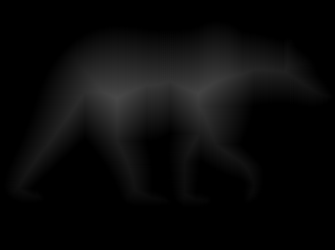
\includegraphics[width=0.3\textwidth]{beard}
            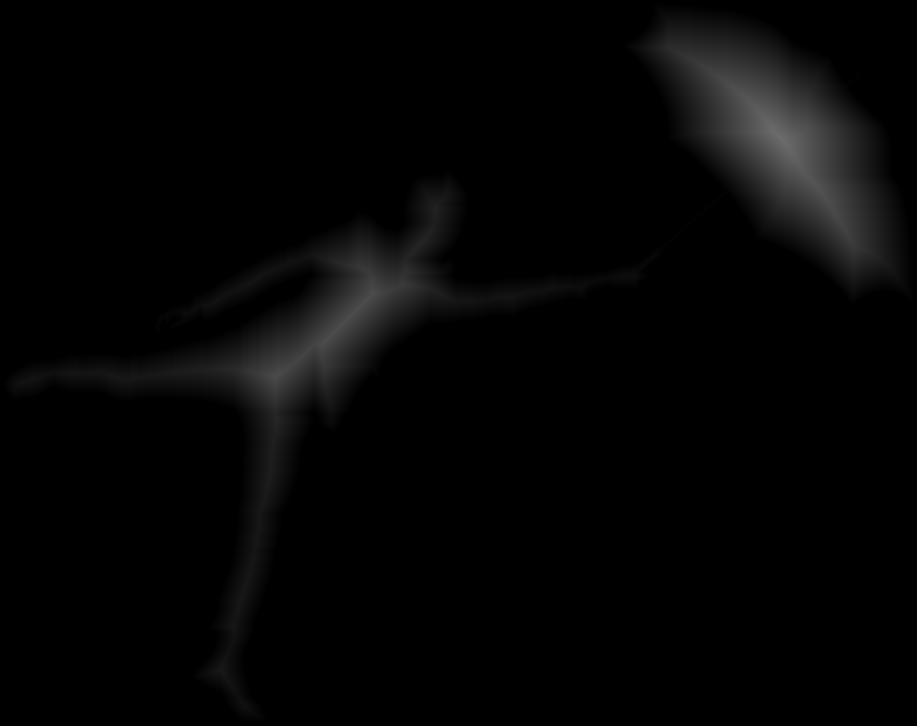
\includegraphics[width=0.3\textwidth]{umbd}
           
  \caption{Distances}
\end{figure}

\begin{figure}
            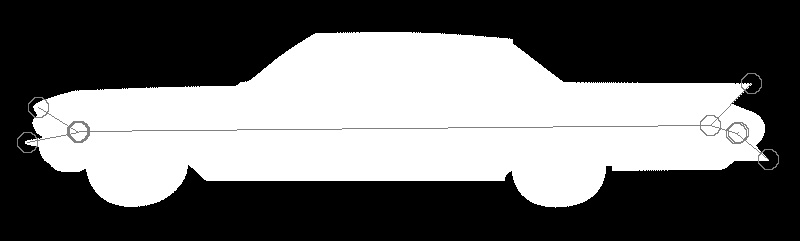
\includegraphics[width=0.9\textwidth]{carskelly}
  \caption{A car skeleton}
\end{figure}

\begin{figure}
            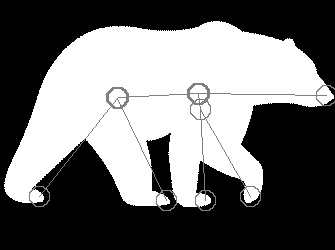
\includegraphics[width=0.9\textwidth]{bearskelly}
  \caption{Bear skeleton}
\end{figure}

\begin{figure}
            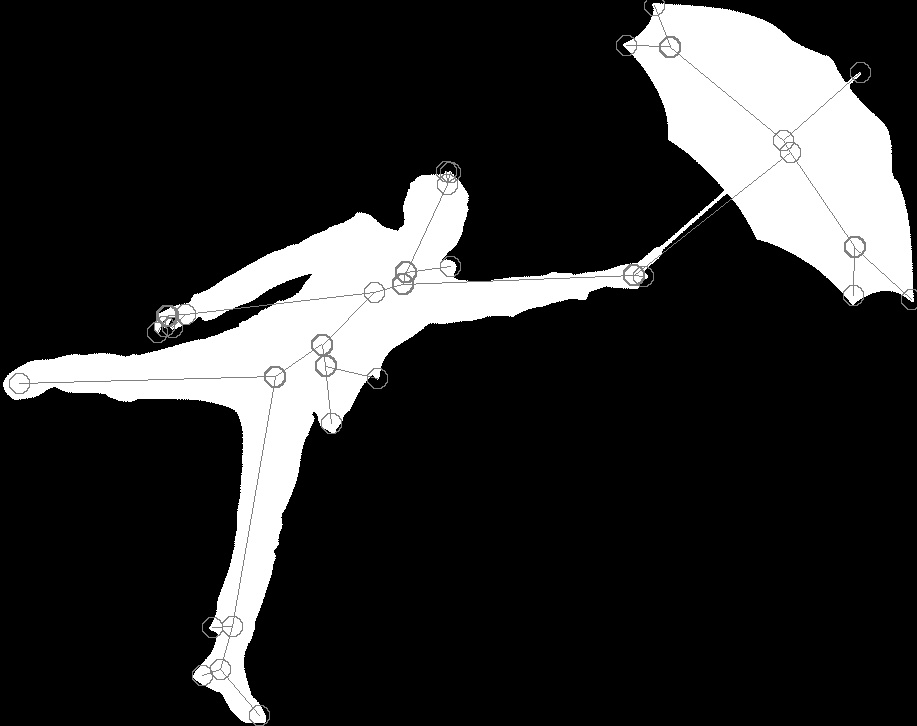
\includegraphics[width=0.9\textwidth]{umbrskelly}
  \caption{Umbrella man skeleton}
\end{figure}
\newpage
\newpage
\pagebreak

\newpage

\begin{figure}
            
\includegraphics[width=0.5\textwidth]{lbp1}
            
\includegraphics[width=0.5\textwidth]{lbp2}
            
\includegraphics[width=0.5\textwidth]{lbp3}
             
\includegraphics[width=0.5\textwidth]{lbp4}
       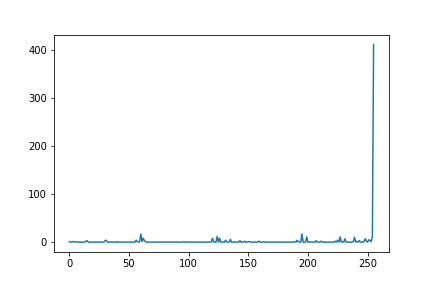
\includegraphics[width=1\textwidth]{histogram}]
           
  \caption{Examples of numbers post LBP and a histogram of some number}
  
\end{figure}            
\end{document}
